\begin{figure}
\centering
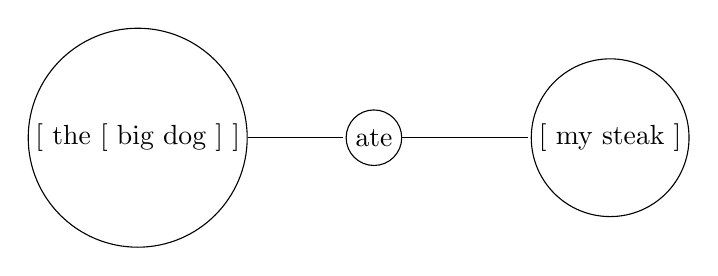
\begin{tikzpicture}[shorten >=1pt, -]
  \tikzstyle{vertex}=[circle,draw=black,minimum size=12pt,inner sep=2pt]
  \node[vertex] (A) at (-3, 0) {
    \Tree [ the [ big dog ] ]
  };
  \node[vertex] (B) at (0, 0) {
    ate
  };
  \node[vertex] (C) at (3, 0) {
    \Tree [ my steak ]
  };

  \draw (A) -- (B);
  \draw (B) -- (C);

\end{tikzpicture}
\caption{An example parsing of an utterance.}
\end{figure}